\paragraph{Locking} The CLM virtual machine uses spin-locks to protect shared data structures between
threads. As described in Section~\ref{sec:implementation}, coordination
operations require synchronization since they need to change node information
and sometimes move nodes between the standard queue and the regular queue.
In order to measure the locking costs of coordination, we measured the following
statistics: \emph{basic locks}, the number of locks acquired that were already
present in the original LM virtual machine and \emph{coordination locks}, the
number of locks acquired for performing coordination operations. We also
measured how often a \texttt{lock()} operation fails on the first attempt, but
such statistics are not represented in the figures below since the values are
too small.

The first program we measured was SSSP, represented in
Fig.~\ref{results:sssp_uspowergrid}. In addition to the Regular and
Coordinated versions, we have the Buffered version where we
optimized the virtual machine to buffer coordination actions before applying
them. The idea is to avoid applying multiple \texttt{set-priority} operations to
the same node during a single node execution. We thus gather the higher priority
values and then perform coordination after the node has executed.
Although the number of locks is significantly reduced, we did not see a
similar performance improvement, since the Buffered version is only
5\% faster than the Coordinated version.

\begin{topfig}
   \begin{center}
      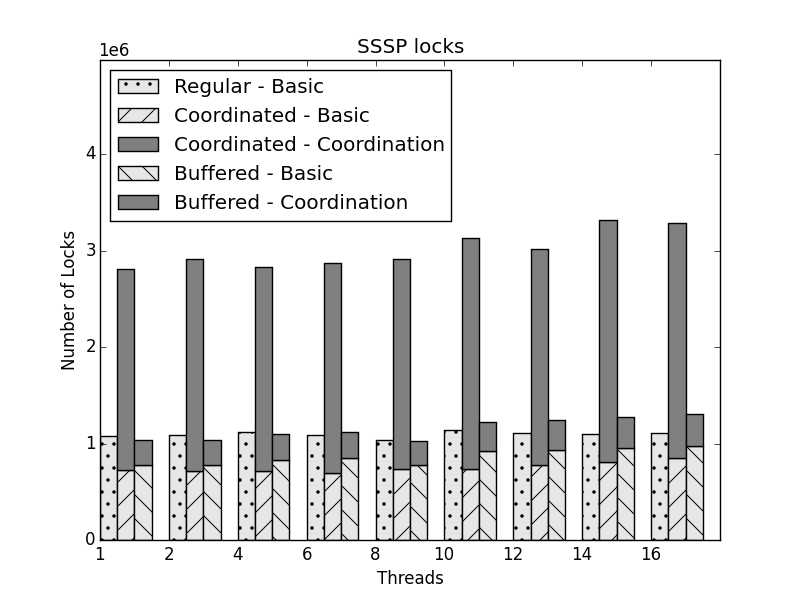
\includegraphics[width=6.5cm]{results/locks/sssp-locks.png}
   \end{center}
  \scap{locks:SSSP}{Locking statistics for SSSP.
     \texttt{Coordinated} refers to the program in
     Fig.~\ref{results:sssp_uspowergrid}, while \texttt{Buffered} is a more
     optimized version of the same program where coordination operations are
     buffered before application.}
\end{topfig}

In Fig.~\ref{locks:HT} we show the lock statistics for HT. We measured the
regular version, the coordinated version and the local-only version as in
Fig.~\ref{results:ht}. There is a slight reduction in number of locks with
coordination and then a further reduction in the local-only version because less
facts are exchanged between threads.

\begin{topfig}
   \begin{center}
      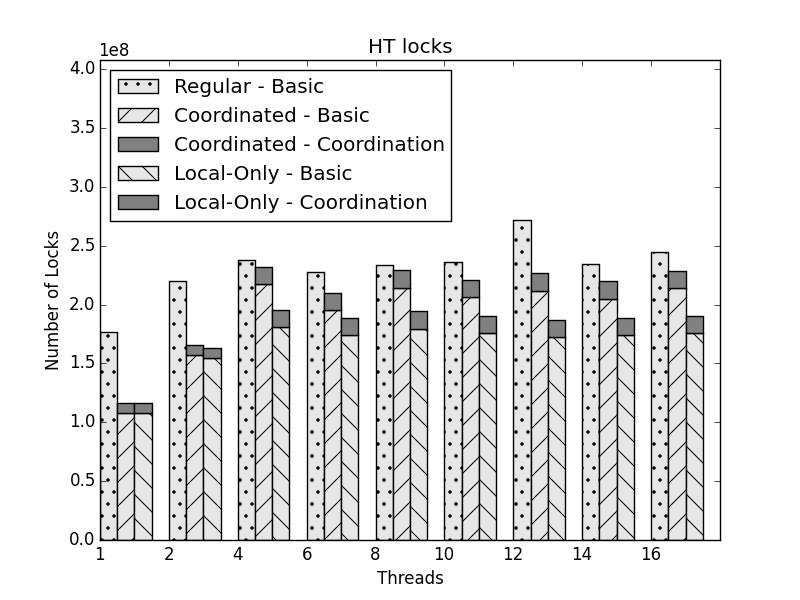
\includegraphics[width=6.5cm]{results/locks/ht-locks.png}
   \end{center}
  \scap{locks:HT}{Locking statistics for HT. Coordination reduces
     the overall number of locks used, while further optimization for locality
     reduces the locks even further.}
\end{topfig}

Finally, in Fig.~\ref{locks:LBP} we present lock statistics for LBP and SBP. LBP
is represented as the Regular bar, while SBP is represented as the Coordinated
bar. We notice that LBP has quite a lot of locking for 1 thread since LBP
is an asynchronous algorithm and tends to be a slow sequential algorithm,
requiring more derivations when using 1 thread. The numbers go down as more
threads are used. For SBP, there is a consistent amount of locking without
little variations between the number of threads used. This is because threads
interact very little with each other and the amount of work to do is the same
for all threads.

\begin{topfig}
   \begin{center}
      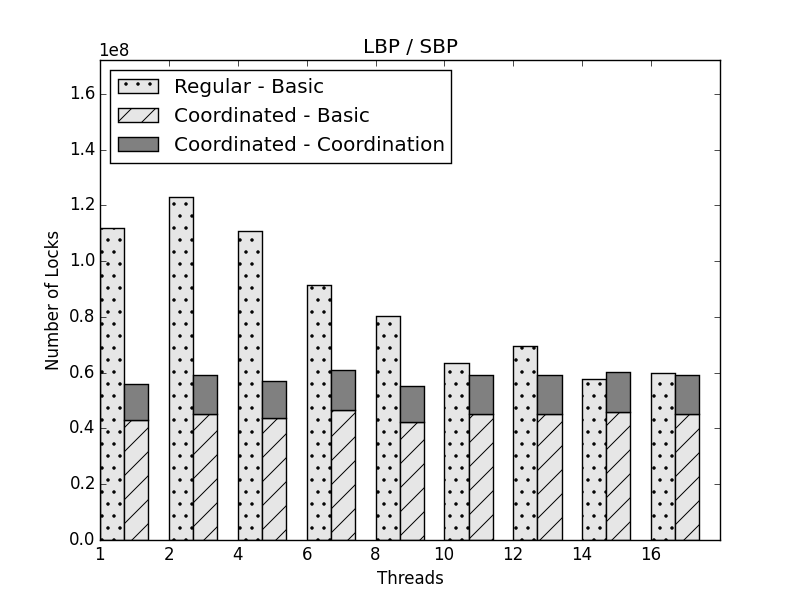
\includegraphics[width=6.5cm]{results/locks/bp.png}
   \end{center}
  \scap{locks:LBP}{Locking statistics for LBP and SBP. Locking is constant for
     SBP because threads do not interact with each other.}
\end{topfig}

\paragraph{Queue Instructions}

We also measured the number of queue instructions required to compute programs.
While the regular queue operations have constant complexity, priority queue
operations are usually logarithmic and require more computation. We counted the
number of instructions required for queue operations during program execution.
Each normal queue operation costs 1 instruction, while priority queue costs as
many \emph{percolate-up}/\emph{percolate-down} instructions are required to maintain the heap property.

Table~\ref{queue_instructions} presents the total queue instructions for several
programs. All the coordinated programs require far more queue instructions than
the regular version. For instance, the coordinated SSSP program requires 4 to 5
times more instructions to perform queue operations. Interestingly, the buffered
version requires even more instructions although it performs less overall
coordination. It is likely that this is due to increased fact computation and
subsequent queue manipulation because coordination operations are buffered.
We argue that the 5\% performance improvement in the
buffered version is due mostly to reduced locking.

For the HT program, the coordinated version requires twice more queue
instructions than the regular version. As expected, the local-only version
requires less queue operations because the number of derived facts is reduced.
The MiniMax program also sees twice as many queue instructions using
coordination. This does not happen with the N Queens program, where the number
of queue instructions is far greater when using coordination, especially when
using a small number of threads. We argue that this happens because higher
priority nodes at the bottom are often added to the priority queue, resulting in
many \emph{percolate-up} operations.

\begin{topfig}
\footnotesize\begin{tabular}{ | l || c | c | c | c | c |}
\hline
\multirow{2}{*}{\textbf{Program}} & \multicolumn{5}{c |}{\textbf{Queue
   Instructions}} \\ \cline{2-6}
& 1 & 2 & 4 & 8 & 16 \\ \hline
\hline
SSSP - Regular & 199K & 201K & 205K & 196K & 207K \\ \hline
SSSP - Coordinated & 964K & 938K & 870K & 886K & 963K \\ \hline
SSSP - Buffered & 1M & 1M & 1M & 1M & 1M \\ \hline
\hline
HT - Buffered & 25M & 32M & 34M & 34M & 36M \\ \hline
HT - Coordinated & 51M & 55M & 85M & 80M & 72M \\ \hline
HT - Local-Only & 51M & 55M & 79M & 74M & 68M \\ \hline
\hline
LBP - Regular & 15M & 17M & 16M & 11M & 8M \\ \hline
SBP - Coordinated & 96M & 97M & 87M & 83M & 77M \\ \hline
\hline
MiniMax - Regular & 16M & 19M & 19M & 19M & 20M \\ \hline
MiniMax - Coordinated & 51M & 51M & 51M & 51M & 52M \\ \hline
\hline
N Queens - Regular & 8K & 15K & 16K & 17K & 20K \\ \hline
N Queens - Coordinated & 57M & 24M & 675K & 145K & 46K \\ \hline
N Queens - Static & 57M & 44M & 1M & 1M & 151K \\ \hline
\hline
\end{tabular}
\scap{queue_instructions}{Number of queue \scare{instructions} per program. An
   operation to a regular queue counts as 1 instruction, while an operation to
   a priority queue costs the number of
   \emph{percolate-up}/\emph{percolate-down} steps performed.}
\end{topfig}

These experiments indicate that handling coordination has a small cost in terms
of synchronization but some cost in terms of queue operations with
up to 5 times more queue instructions when using priority queues.
Since coordination reduces the number of facts derived due to better scheduling
decisions, the costs of manipulating priority queues become irrelevant.

